
\documentclass[a4paper,11pt]{article}
\usepackage{graphicx}
\usepackage{caption}
\captionsetup{justification=centering,font={small,sf}}
\usepackage{pgfplots}
\pgfplotsset{compat=1.3}
\usepackage{hyperref}
\usepackage{siunitx}
\usepackage{commath}
\usepackage{mathtools}
\usepackage{color}
\usepackage{listings}

\usepackage{caption}
\usepackage{subcaption}


\usetikzlibrary{plotmarks}

\definecolor{javared}{rgb}{0.6,0,0} % for strings
\definecolor{javagreen}{rgb}{0.25,0.5,0.35} % comments
\definecolor{javapurple}{rgb}{0.5,0,0.35} % keywords
\definecolor{javadocblue}{rgb}{0.25,0.35,0.75} % javadoc
 
\lstset{language=Java,
basicstyle=\ttfamily,
keywordstyle=\color{javapurple}\bfseries,
stringstyle=\color{javared},
commentstyle=\color{javagreen},
morecomment=[s][\color{javadocblue}]{/**}{*/},
tabsize=4,
showspaces=false,
showstringspaces=false}

\setlength{\voffset}{-25mm}
\setlength{\hoffset}{-10mm}
\setlength{\oddsidemargin}{0mm}
\setlength{\evensidemargin}{0mm}

\setlength{\marginparwidth}{0mm}
\addtolength{\textwidth}{50mm}
\addtolength{\textheight}{55mm}



\usepackage{color} %red, green, blue, yellow, cyan, magenta, black, white
\definecolor{mygreen}{RGB}{28,172,0} % color values Red, Green, Blue
\definecolor{mylilas}{RGB}{170,55,241}



\lstset{language=Matlab,%
    %basicstyle=\color{red},
    breaklines=true,%
    morekeywords={matlab2tikz},
    keywordstyle=\color{blue},%
    morekeywords=[2]{1}, keywordstyle=[2]{\color{black}},
    identifierstyle=\color{black},%
    stringstyle=\color{mylilas},
    commentstyle=\color{mygreen},%
    showstringspaces=false,%without this there will be a symbol in the places where there is a space
    numbers=left,%
    numberstyle={\tiny \color{black}},% size of the numbers
    numbersep=9pt, % this defines how far the numbers are from the text
    emph=[1]{for,end,break},emphstyle=[1]\color{red}, %some words to emphasise
    %emph=[2]{word1,word2}, emphstyle=[2]{style},    
}










\begin{document}

\begin{center}
\Large{\textbf{CO24: Chaos}}\\ 
\vspace{1em}
\large{A. Vitarana (pemb5671)}\\
\large{Pembroke College}
\end{center}

\section{Abstract}
We calculate solutions of the Lorentz system using the fourth-order Runga-Kutta algorithm, given initial conditions and parameters for the Lorenz equations. Plotting the trajectory of the variables, it is clear the system is sensitive to changes in its initial conditions in certain regimes of the parameters; the system exhibits chaotic behaviour with parameters set close to a=10, b=8/3 and r=28. 


\section{Introduction}

The Lorenz equations are three ordinary differential equations that form the Lorentz model. The Lorenz equations of the time-dependent variables $y_{1}$, $y_{2}$ and $y_{3}$ are:

\begin{eqnarray}
   \dod{y_{1}}{t} &=& a(y_{2}-y_{1})        \\
   \dod{y_{2}}{t} &=& ry_{1} -y_{2}-y_{1}y_{3}   \\ 
   \dod{y_{3}}{t} &=& y_{2}y_{1} - by_{3} , 
\label{eqn:model_1}
\end{eqnarray}

where $a$, $r$, and $b$ are constants.\\
\\
These equations can be used as a simplified model of atmospheric conduction, with each variable describing properties of the fluid in the Rayleigh-Bénard experiment, and they can be derived from the Navier-Stokes equations, the equation for heat conduction and the continuity equation [1]. Physically, $y_{1}$ is proportional to the rate of convection, $y_{2}$ to the temperature difference between currents and $y_{3}$ is the temperature difference between the top and the bottom of the fluid, where $a$ is the Prandtl number, $r$ is the Rayleigh number and $b$ is a geometric factor [2]. \\
\\

The set of equations has three stationary solutions:

\begin{equation}
y_{1} = y_{2} = \pm \sqrt{b(r-1)} , y_{3} = (r-1)
\end{equation}
\begin{equation}
y_{1} = y_{2} = y_{3} = 0, 
\end{equation}
\\
The approach to these solutions from an arbitrary starting point are dependent on the regime of r [3].

\begin{enumerate}
\item 
If $r<1$ the only real stationary point is the origin
\item 
If $r>1$ all three stationary points exist. However, the origin is unstable and so you will never reach it unless
you start exactly on it. As r increases, there is a higher degree of uncertainty in the system.
\begin{enumerate}
\item 
If $r<1$ is less than about 24 the system will converge to one of the two stationary points not found at the origin.
\item 
If $r>1$ is greater than about 24, the system will not converge to either solution and will move between the two fixed points in space. The behaviour is bounded but non-periodic.

\end{enumerate}


\end{enumerate}




\section{Methods}



These equations are coupled first order differential equation and numerical solutions are much easier to obtain than attempts to solve analytically through decouple the solutions or particular integrals and complementary functions. Runge-Kutta methods are iterative methods of approximately solving ordinary equations using small time steps. The Runge-Kutta method implemented in this program was the fourth-order method (RK4). The equations given in 1-3 are in the form,

\begin{equation}
\dod{y_i}{t} = f(y_{1},y_{2},y_{3}).
\end{equation}
\\
Defining a small time interval $\delta t$, the value of the $y_{i}$ can be iteratively calculated at time steps of $\delta t$. Referring to the mth intermediate point in our calculation as $y_{i,m}$ and $f_{i,m}$, the RK4 iteration steps are:

\begin{enumerate}
\item 
Calculate $f_{i,0}$ using $y_{i,0}$ 
\item 
Calculate $f_{i,1}$ using $y_{i,1} = y_{i,0} + \frac{y_{i,0}\delta t}{2}$ 
\item 
Calculate $f_{i,2}$ using $y_{i,2} = y_{i,1} + \frac{y_{i,1}\delta t}{2}$ 
\item 
Calculate $f_{i,3}$ using $y_{i,3} = y_{i,2} + y_{i,2}\delta t$ 
\item 
$y_{i,4} = y_{i,0} + \frac{(f_{i,0}+2f_{i,1}+2f_{i,2}+f_{i,3})\delta t}{6}$ 

\end{enumerate}



The values $y_{i,4}$ then become $y_{i,0}$ in the next step and the value of $y_{i,n}$, where $n=4m$, corresponds to the value of $y_{i}$ at time, $t = m\delta t$. The initial conditions of the system $y_{i,0}$ and the parameters of the system, $a$, $b$ and $r$ can be varied.\\
\\
Although faster methods exist, Runge-Kutta methods nearly always work and hence are often used to produce a numerical solution [4]. Runge-Kutta algorithms are derived from Simpson's rule and use varying subintervals depending on their order; the fourth order algorithm gives the best balance between accuracy and computational effort  [5]. These algorithms are better approximations of solutions than Euler's method due to the use of higher order terms which reduces truncation error, but they require more computational power.\\
\\

\section{Analysis and Results}

\subsection{Different Regimes of r}

We fix the values of the parameters $a=10$ and $b=8/3$. Also, to compare different regimes we fix the initial conditions $y_{1,0}=1$, $y_{2,0}=2$ and $y_{3,0}=3$ and the solutions are evaluated over $n=500$ time steps, $\delta t=0.05$.


\subsubsection{$r<1$}

Setting $r=0$, from figure 1(a), we observe that the values of $y_{1}$, $y_{2}$ and $y_{3}$ converge to zero, which we expect since the only real stationary point in this regime is the origin. Figure 1(b) shows the relation between variables $y_{2}$ and $y_{3}$; their behaviour towards converging at the origin is non-chaotic.





    
\begin{figure}
     \centering
     \begin{subfigure}[b]{0.45\textwidth}
         \centering
         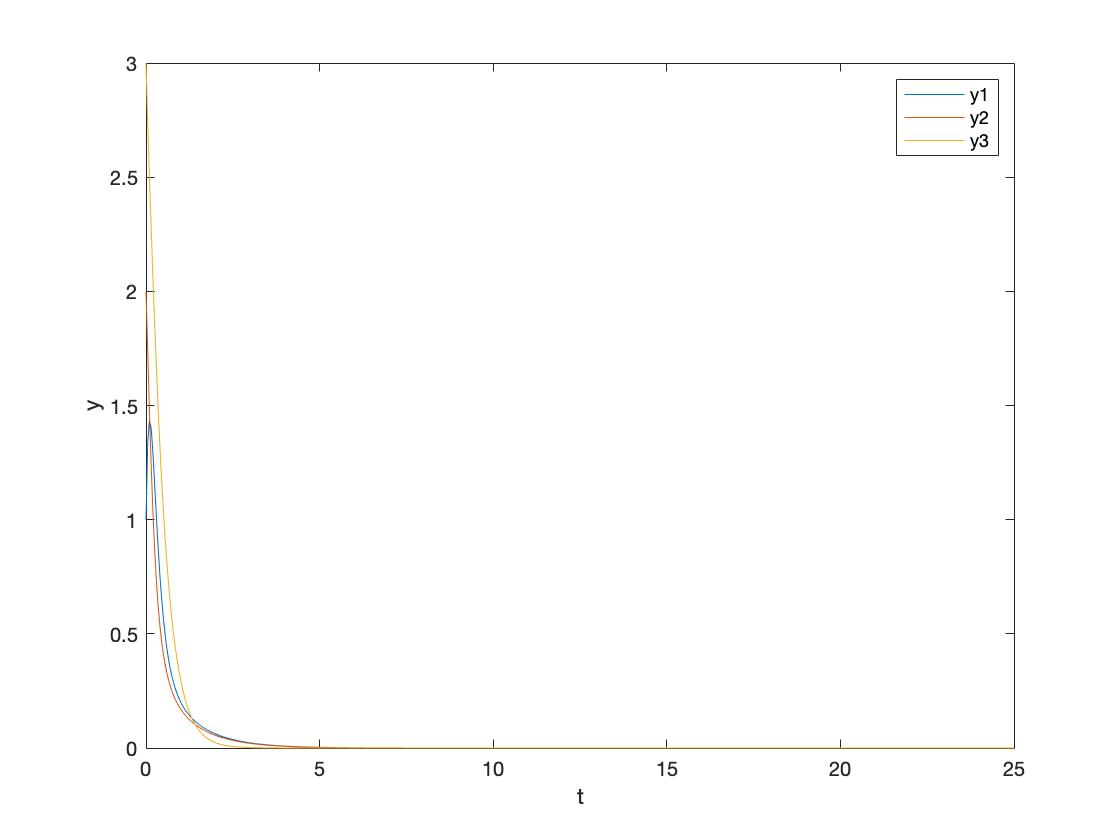
\includegraphics[width=\textwidth]{r0_y123_time}
         \caption{Graph of $y_{1}$, $y_{2}$ and $y_{3}$ against time}
         \label{fig:y equals x}
     \end{subfigure}
     \hfill
     \begin{subfigure}[b]{0.45\textwidth}
         \centering
         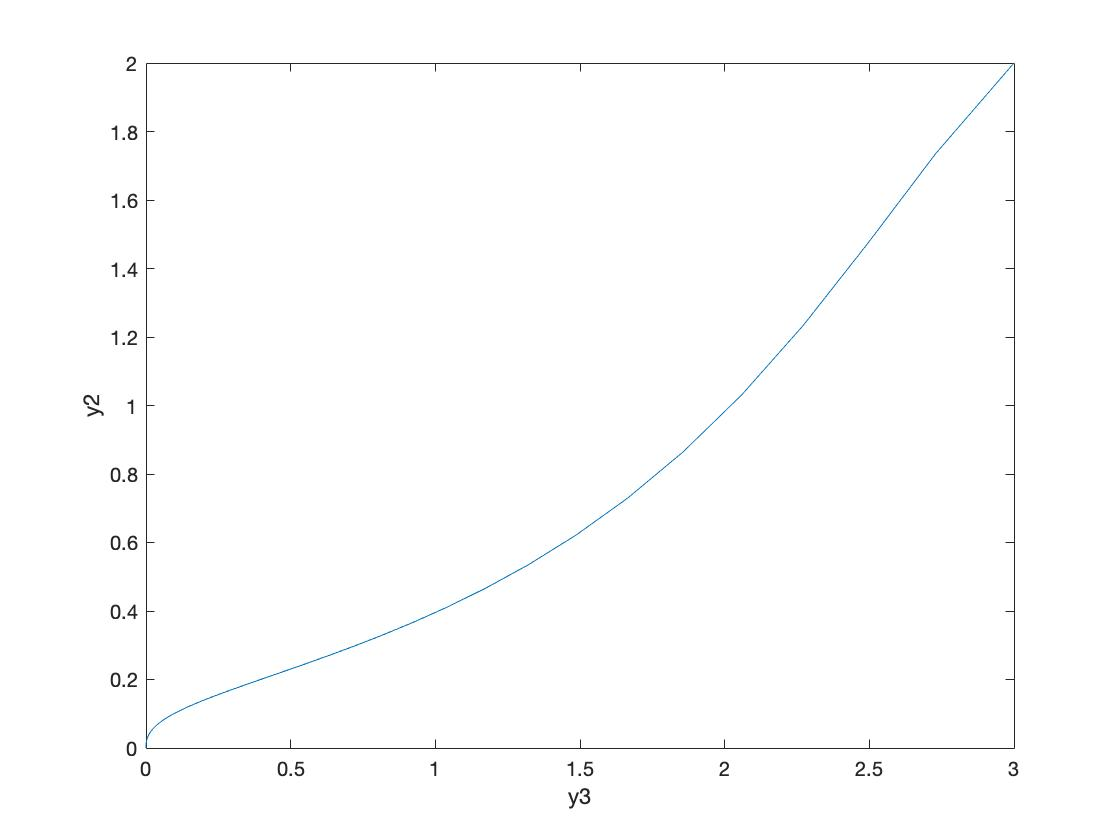
\includegraphics[width=\textwidth]{r0_y2_y3}
         \caption{Graph of $y_{2}$ against $y_{3}$}
         \label{fig:three sin x}
     \end{subfigure}
        \caption{$r=0$}
        \label{fig:r=0}
\end{figure}

\subsubsection{$1<r<24$}

Setting $r=15$, from figure 2(a), we observe that the values of $y_{1}$, $y_{2}$ and $y_{3}$ converge to one of the solutions, not including the origin, unless the initial conditions start at the origin since it is unstable. Figure 2(b) shows this convergence is a reached by spiralling around the solution.


\begin{figure}
     \centering
     \begin{subfigure}[b]{0.45\textwidth}
         \centering
         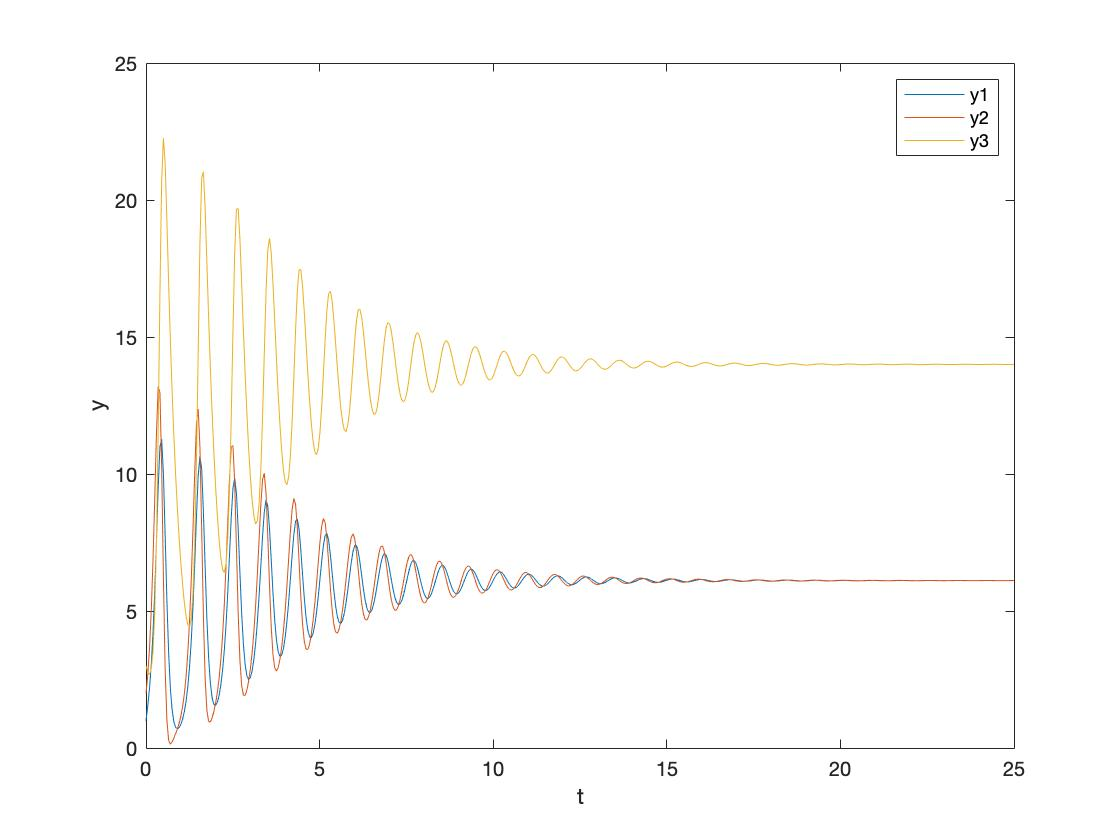
\includegraphics[width=\textwidth]{r15_y123_time}
         \caption{Graph of $y_{1}$, $y_{2}$ and $y_{3}$ against time}
         \label{fig:y equals x}
     \end{subfigure}
     \hfill
     \begin{subfigure}[b]{0.45\textwidth}
         \centering
         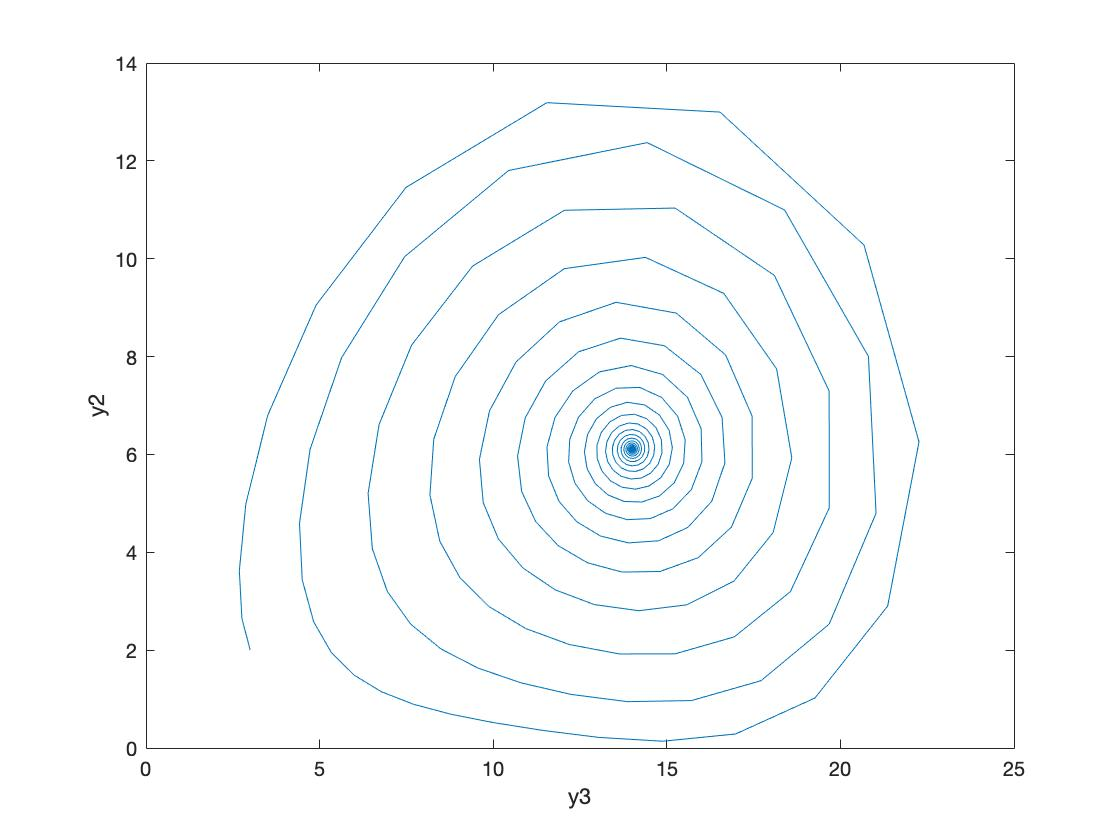
\includegraphics[width=\textwidth]{r15_y2_y3}
         \caption{Graph of $y_{2}$ against $y_{3}$}
         \label{fig:three sin x}
     \end{subfigure}
        \caption{$r=15$}
        \label{fig:r=15}
\end{figure}

\begin{figure}
     \centering
     \begin{subfigure}[b]{0.45\textwidth}
         \centering
         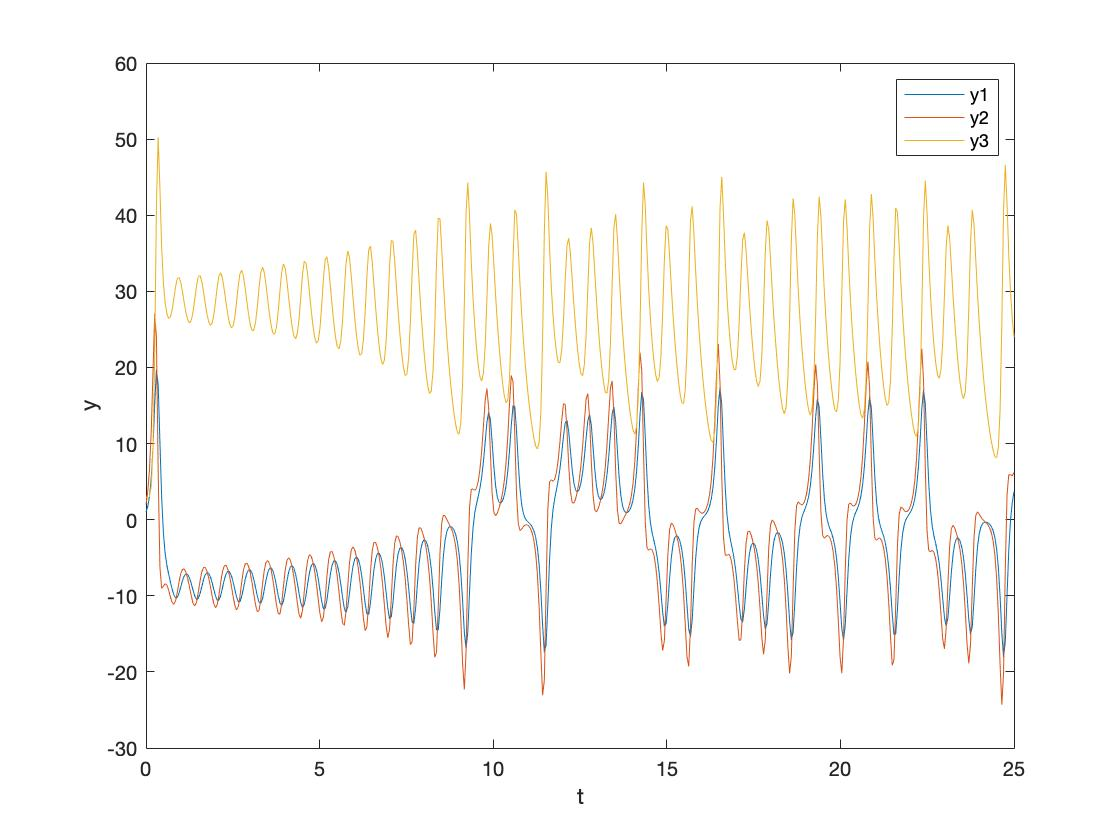
\includegraphics[width=\textwidth]{r30_y123_time}
         \caption{Graph of $y_{1}$, $y_{2}$ and $y_{3}$ against time}
         \label{fig:y equals x}
     \end{subfigure}
     \hfill
     \begin{subfigure}[b]{0.45\textwidth}
         \centering
         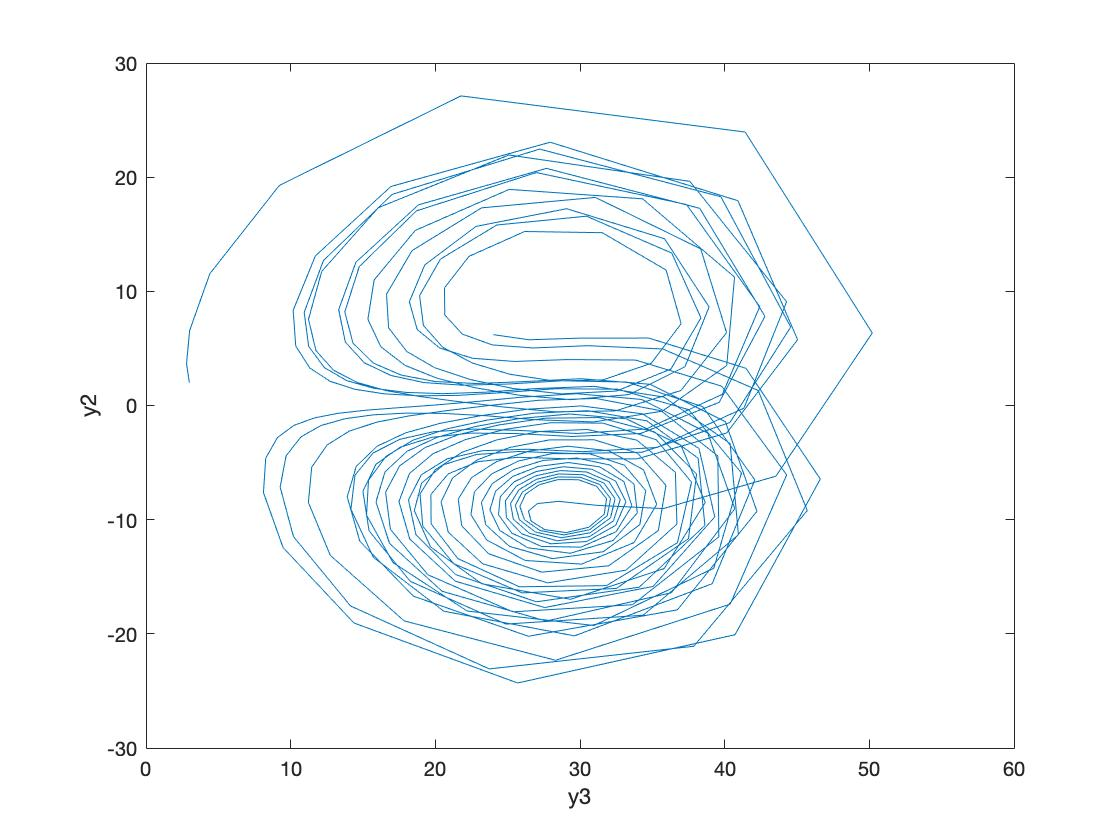
\includegraphics[width=\textwidth]{r30_y2_y3}
         \caption{Graph of $y_{2}$ against $y_{3}$}
         \label{fig:three sin x}
     \end{subfigure}
        \caption{$r=30$}
        \label{fig:r=30}
\end{figure}


\subsubsection{$r>24$}

Setting $r=30$, from figure 3(a), we observe that the values of $y_{1}$, $y_{2}$ and $y_{3}$ do not converge to one of the solutions, but instead wanders between the two solutions that are not the unstable origin. Figure 3(b) shows this convergence is a reached by spiralling around the solution.
\\

This is a strange attractor, since the solutions are bounded but non-periodic. Plotting all three coordinates against each other, a more intuitive image of the Lorentz attractor can be viewed as in figure 4.









\begin{figure}

     \centering
         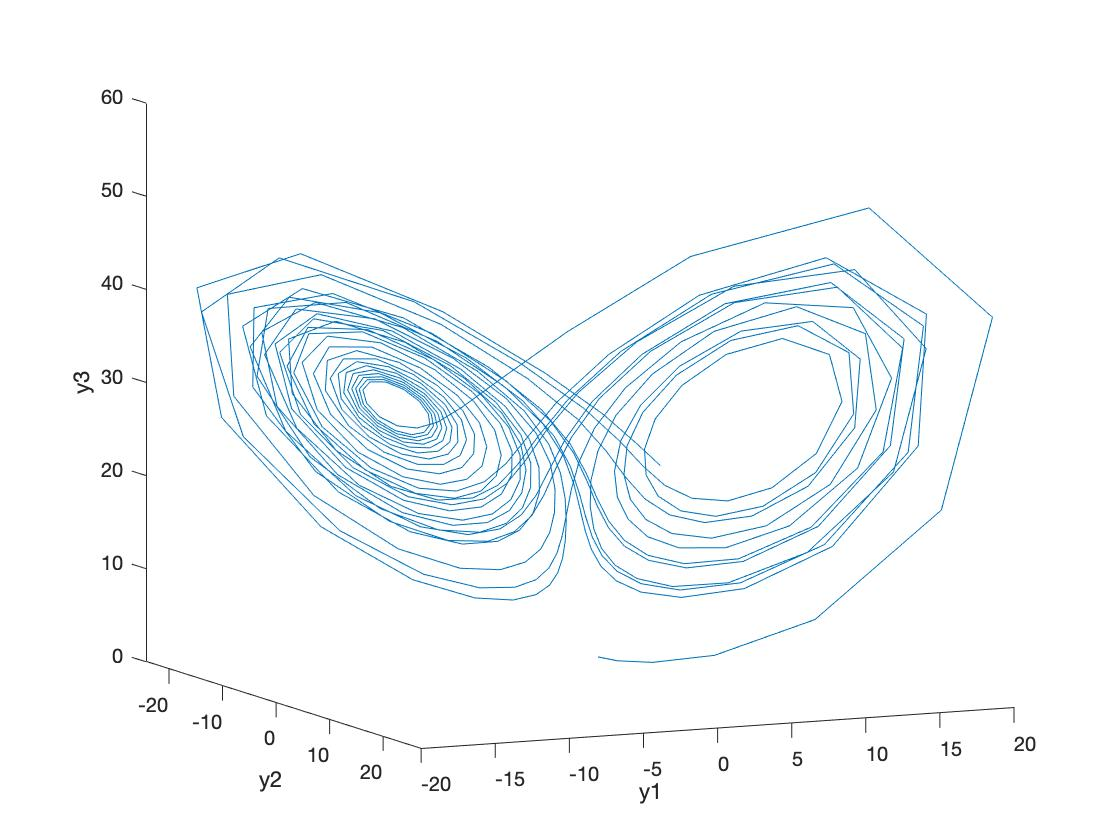
\includegraphics[width=0.8\textwidth]{r30_3D}
         \caption{3D plot of $y_{1}$, $y_{2}$ and $y_{3}$ at $r=30$}

\end{figure}



\subsection{Chaotic Behaviour: `the weather forecasting' phenomena}

From \S 4.1.3, we observe what seems to be chaotic behaviour. To analyse this behaviour we fix the values of the parameters $a=10$, $b=8/3$ and $r=28$, but slightly change the initial conditions  $y_{1,0}$, $y_{2,0}$ and $y_{3,0}$. As before, the solutions are evaluated over $n=500$ time steps, $\delta t=0.05$. Initially, we set the initial conditions $y_{1,0}=4$, $y_{2,0}=5$ and $y_{3,0}=6$, which we call these the real conditions. The time-evolution of the variables are compared to initial conditions $y_{1,0}=4.01$, $y_{2,0}=5.01$ and $y_{3,0}=6.01$, which we call a 'small measurement error'.\\
\\
Focusing on the time-evolution of $y_{1}$, Figure 5 shows that the slight change in initial conditions leads to a similar initial time evolution. However, after a short period of time the solutions separate and begin to wander about the two solutions following different paths. This demonstrates deterministic chaotic behaviour, since the present determines the future but the approximate present does not approximately determine the future. Since, weather systems can be approximated by the Lorentz model this demonstrates the difficulties of predicting the weather; small measurement errors will lead to vastly different outcomes.

\begin{figure}

     \centering
         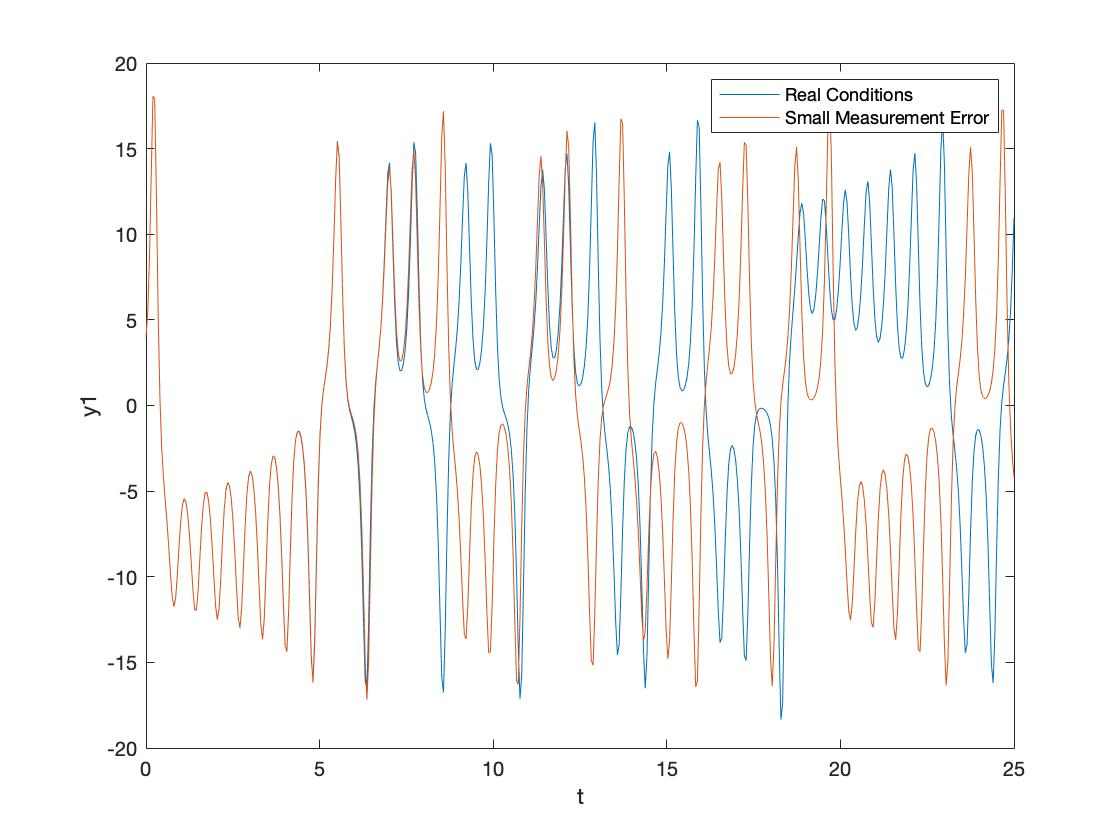
\includegraphics[width=0.8\textwidth]{r28_y1_timeX}
         \caption{$y_{1}$ against time with a 'small measurement error' in initial conditions}

\end{figure}



\clearpage

\section{Conclusions}

The Lorentz system demonstrates chaotic behaviour in the regime $r>24$, since a small change in the initial conditions of the system drastically changes the time-evolution of the system. The Lorentz attractor is observed, since the system is bounded by two solutions, but does not converge to either. In the approximately the regime $1<r<24$, the system will converge to one of the two solutions, which are not the origin, depending upon initial conditions. In the regime, $r<1$, the system will converge to the solution at the origin.\\
\\
The RK4 method offers a clear visualisation of the chaotic behaviour observed. However, since the RK4 method is an iterative method it propagates error. This is particularly unhelpful when studying chaos as the system is sensitive to small changes and therefore the numerical solution obtained by the RK4 method is likely to be vastly different from the actual solution after a long period of time; a small local error develops into a large global error. Another disadvantage in my ODE solver program was the use of equally spaced time intervals as at turning points the RK4 method is more inaccurate. Combing the RK4 method with intelligent adaptive step-size routine would increase the accuracy of the solution; MatLab has an inbuilt ode45 function that uses RK4 with changing time-steps. For systems with a large numbers of coupled equations, this adaptive step-size is particularly important. The ODE solver is extremely versatile and slight modifications to the program allow the higher order ODEs to be solved, such as a damped oscillator. 




\begin{thebibliography}{9}
\bibitem{Chaos} Schuster\ H.\ G. (1988). \emph{Deterministic chaos: an introduction}, 2nd Ed. Darmstadt: betz-druck gmbh, p 223-225.

\bibitem{Lab Script} Weisstein, E. (2018). \emph{CO24: chaos} [Accessed 24 January 2020] Available at: http://mathworld.wolfram.com/LorenzAttractor.html

\bibitem{Lab Script} (2018). \emph{Lorentz Attractor} [Accessed 24 January 2020] Available at: https://www-teaching.physics.ox.ac.uk
\bibitem{RK4} Press\ W.\ H. et al. (2007). \emph{Numerical Recipes: the Art of Scientific Computing}, 3rd Ed. Cambridge: Cambridge University Press, p 908. 
\bibitem{RK4} O'Hare\ A. (2005). \emph{Numerical Methods for Physicists}, Oxford Physics, p 69. 
\end{thebibliography}

\clearpage





\appendix
\renewcommand\thesection{Appendix \Alph{section}}

\section{ODE Solver}
\begin{lstlisting}
function [y] = ode_solve_rk(f1, f2, f3 , y0 , t)
% Author: Aaron Vitarana, Date: 22/01/2020
%
% Solve ODE problems using Runge-Kutta algorithm.
% 
% Input:
% * f1, f2, f3: functions that receive current states of y1, y2 and y3
% * y0: the initial state of the system, given in a column matrix (3 x 1).
% * t: vector of equally spaced position/time steps with length N where the values of y will be returned.
%
% Output:
% y: (3 x N) matrix that contains the values of y at every position/time
% step and columns correspond to the position/time and rows to the element of y.


% setting up initial vector and filling it with the initial conditions
y = zeros(3, length(t))
y(1, 1) = y0(1, 1); 
y(2, 1) = y0(2,1);
y(3, 1) = y0(3,1);

% determining time step
dt = abs(t(2) - t(1));

    
for a = 1:(length(t)-1) %iterate through all values of t except the largest value
    k1 = f1(y(1,a), y(2,a), y(3,a));
    l1 = f2(y(1,a), y(2,a), y(3,a));
    m1 = f3(y(1,a), y(2,a), y(3,a));
    k2 = f1(y(1,a) + 0.5*k1*dt, y(2,a) + 0.5*l1*dt, y(3,a) + 0.5*m1*dt);
    l2 = f2(y(1,a) + 0.5*k1*dt, y(2,a) + 0.5*l1*dt, y(3,a) + 0.5*m1*dt);
    m2 = f3(y(1,a) + 0.5*k1*dt, y(2,a) + 0.5*l1*dt, y(3,a) + 0.5*m1*dt);
    k3 = f1(y(1,a) + 0.5*k2*dt, y(2,a) + 0.5*l2*dt, y(3,a) + 0.5*m2*dt);
    l3 = f2(y(1,a) + 0.5*k2*dt, y(2,a) + 0.5*l2*dt, y(3,a) + 0.5*m2*dt);
    m3 = f3(y(1,a) + 0.5*k2*dt, y(2,a) + 0.5*l2*dt, y(3,a) + 0.5*m2*dt);
    k4 = f1(y(1,a) + k3*dt, y(2,a) + l3*dt, y(3,a) + m3*dt);
    l4 = f2(y(1,a) + k3*dt, y(2,a) + l3*dt, y(3,a) + m3*dt);
    m4 = f3(y(1,a) + k3*dt, y(2,a) + l3*dt, y(3,a) + m3*dt);
    
    y(1, a+1) = y(1, a) + (k1 + 2*k2 + 2*k3 + k4)*dt/6;
    y(2, a+1) = y(2, a) + (l1 + 2*l2 + 2*l3 + l4)*dt/6;
    y(3, a+1) = y(3, a) + (m1 + 2*m2 + 2*m3 + m4)*dt/6;
end

end
\end{lstlisting}

\clearpage

\section{Lorenz Equations}
\begin{lstlisting}
function [y] = solve_lorenz(y0 , a , b , r , t)
% Author: Aaron Vitarana, Date: 22/01/2020
% Solve Lorenz equations using the implemented ODE solver.
% Dedicated to Anna
% Input:
% * y0: a column vector of the starting point with size (3 x 1)
% * a, b, r: parameters of the Lorenz equations
% * t: an N?element vector of time/position steps where y will be calculated
%
% Output:
% * y: a (3 x N) matrix that contains the values of y for every time step
 
% defining Lorenz functions
f1 = @(y1, y2, y3) (a*(y2-y1))
f2 = @(y1, y2, y3) (r*y1-y2-y1*y3)
f3 = @(y1, y2, y3) (y1*y2-b*y3)
 
 
% calls Runga-Kutta function to solve ODEs
% returns y: (M x N) matrix that contains the values of y at every position/time
% step and columns correspond to the position/time and rows to the element of y.
[y] = ode_solve_rk(f1, f2, f3, y0 , t)
 
end

\end{lstlisting}








\end{document}     
